% slides.tex — UNISTRA NLP 2026 Lecture: Applied NLP
% "A Practical Journey Through NLP"
% Compile with: pdflatex slides.tex (twice for frame numbers)

\documentclass[aspectratio=169,11pt]{beamer}

\IfFileExists{beamerthememedievalnlp.sty}{%
  \usetheme{medievalnlp}%
}{%
  \usetheme{default}%
  \usepackage{xcolor}%
  \definecolor{bglight}{HTML}{F5EFE6}%
  \definecolor{bgcard}{HTML}{EDE8E0}%
  \definecolor{bgaccent}{HTML}{E5DDD3}%
  \definecolor{textdark}{HTML}{2C2421}%
  \definecolor{textsecond}{HTML}{4A4340}%
  \definecolor{textmuted}{HTML}{8A7B70}%
  \definecolor{coral}{HTML}{E07850}%
  \definecolor{corallight}{HTML}{F0A080}%
  \definecolor{coraldark}{HTML}{C05830}%
  \definecolor{gold}{HTML}{D4A855}%
  \definecolor{green}{HTML}{5A8A5A}%
  \definecolor{blue}{HTML}{5B8DB8}%
  \setbeamercolor{background canvas}{bg=bglight}%
  \setbeamercolor{normal text}{fg=textdark}%
  \setbeamercolor{structure}{fg=coral}%
  \setbeamertemplate{navigation symbols}{}%
  \newcommand{\highlight}[1]{\textcolor{coral}{#1}}%
  \newcommand{\muted}[1]{\textcolor{textmuted}{#1}}%
  \newcommand{\gold}[1]{\textcolor{gold}{#1}}%
  \newcommand{\green}[1]{\textcolor{green}{#1}}%
  \newcommand{\cmark}[1]{\hfill{\tiny\color{textmuted}#1}}%
  \newcommand{\citeslide}[1]{{\tiny\color{textmuted}#1}}%
  \newcommand{\coralrule}{\textcolor{coral}{\rule{\textwidth}{1pt}}}%
}

\usepackage{graphicx}
\usepackage{hyperref}
\hypersetup{colorlinks=true,linkcolor=coral,urlcolor=corallight}
\usepackage{booktabs}
\usepackage{tikz}
\usetikzlibrary{shapes,arrows.meta,positioning,calc,decorations.pathreplacing,backgrounds,matrix}
\usepackage{pgfplots}
\pgfplotsset{compat=1.18}
\usepackage{listings}
\lstset{
  basicstyle=\ttfamily\scriptsize\color{textdark},
  backgroundcolor=\color{bgaccent},
  keywordstyle=\color{coral},
  stringstyle=\color{gold},
  commentstyle=\color{textmuted},
  frame=none,
  breaklines=true
}

% --- Round 1 readability refinements ---
% Higher-contrast emphasis color for projector readability.
\definecolor{gold}{HTML}{D95F02}
\setbeamercolor{framesubtitle}{fg=textsecond}
\setbeamertemplate{frametitle}{%
  \vspace{0.45cm}%
  \noindent\insertframetitle%
  \par%
  \ifx\insertframesubtitle\empty\else%
    \vspace{0.06cm}%
    {\usebeamerfont{framesubtitle}\usebeamercolor[fg]{framesubtitle}\insertframesubtitle}%
  \fi%
  \vspace{0.18cm}%
}
\renewcommand{\gold}[1]{\textcolor{gold}{#1}}
% Keep citations away from the page number area.
\renewcommand{\cmark}[1]{%
  \hfill{\tiny\color{textmuted}\mbox{#1\hspace{2.2em}}}%
}

% ── Metadata ──
\title{Applied NLP}
\subtitle{From Text to Intelligence}
\author{Roman Jurowetzki}
\institute{Aalborg University / University of Strasbourg}
\date{February 10--12, 2026 \enspace\textbullet\enspace University of Strasbourg}

\begin{document}

% ═══════════════════════════════════════════════════════════════
% SECTION 0: TITLE & ROADMAP
% ═══════════════════════════════════════════════════════════════

% --- Slide 1: Title ---
\begin{frame}[plain,noframenumbering]
  \IfFileExists{figures/generated/title.png}{%
    \begin{center}
      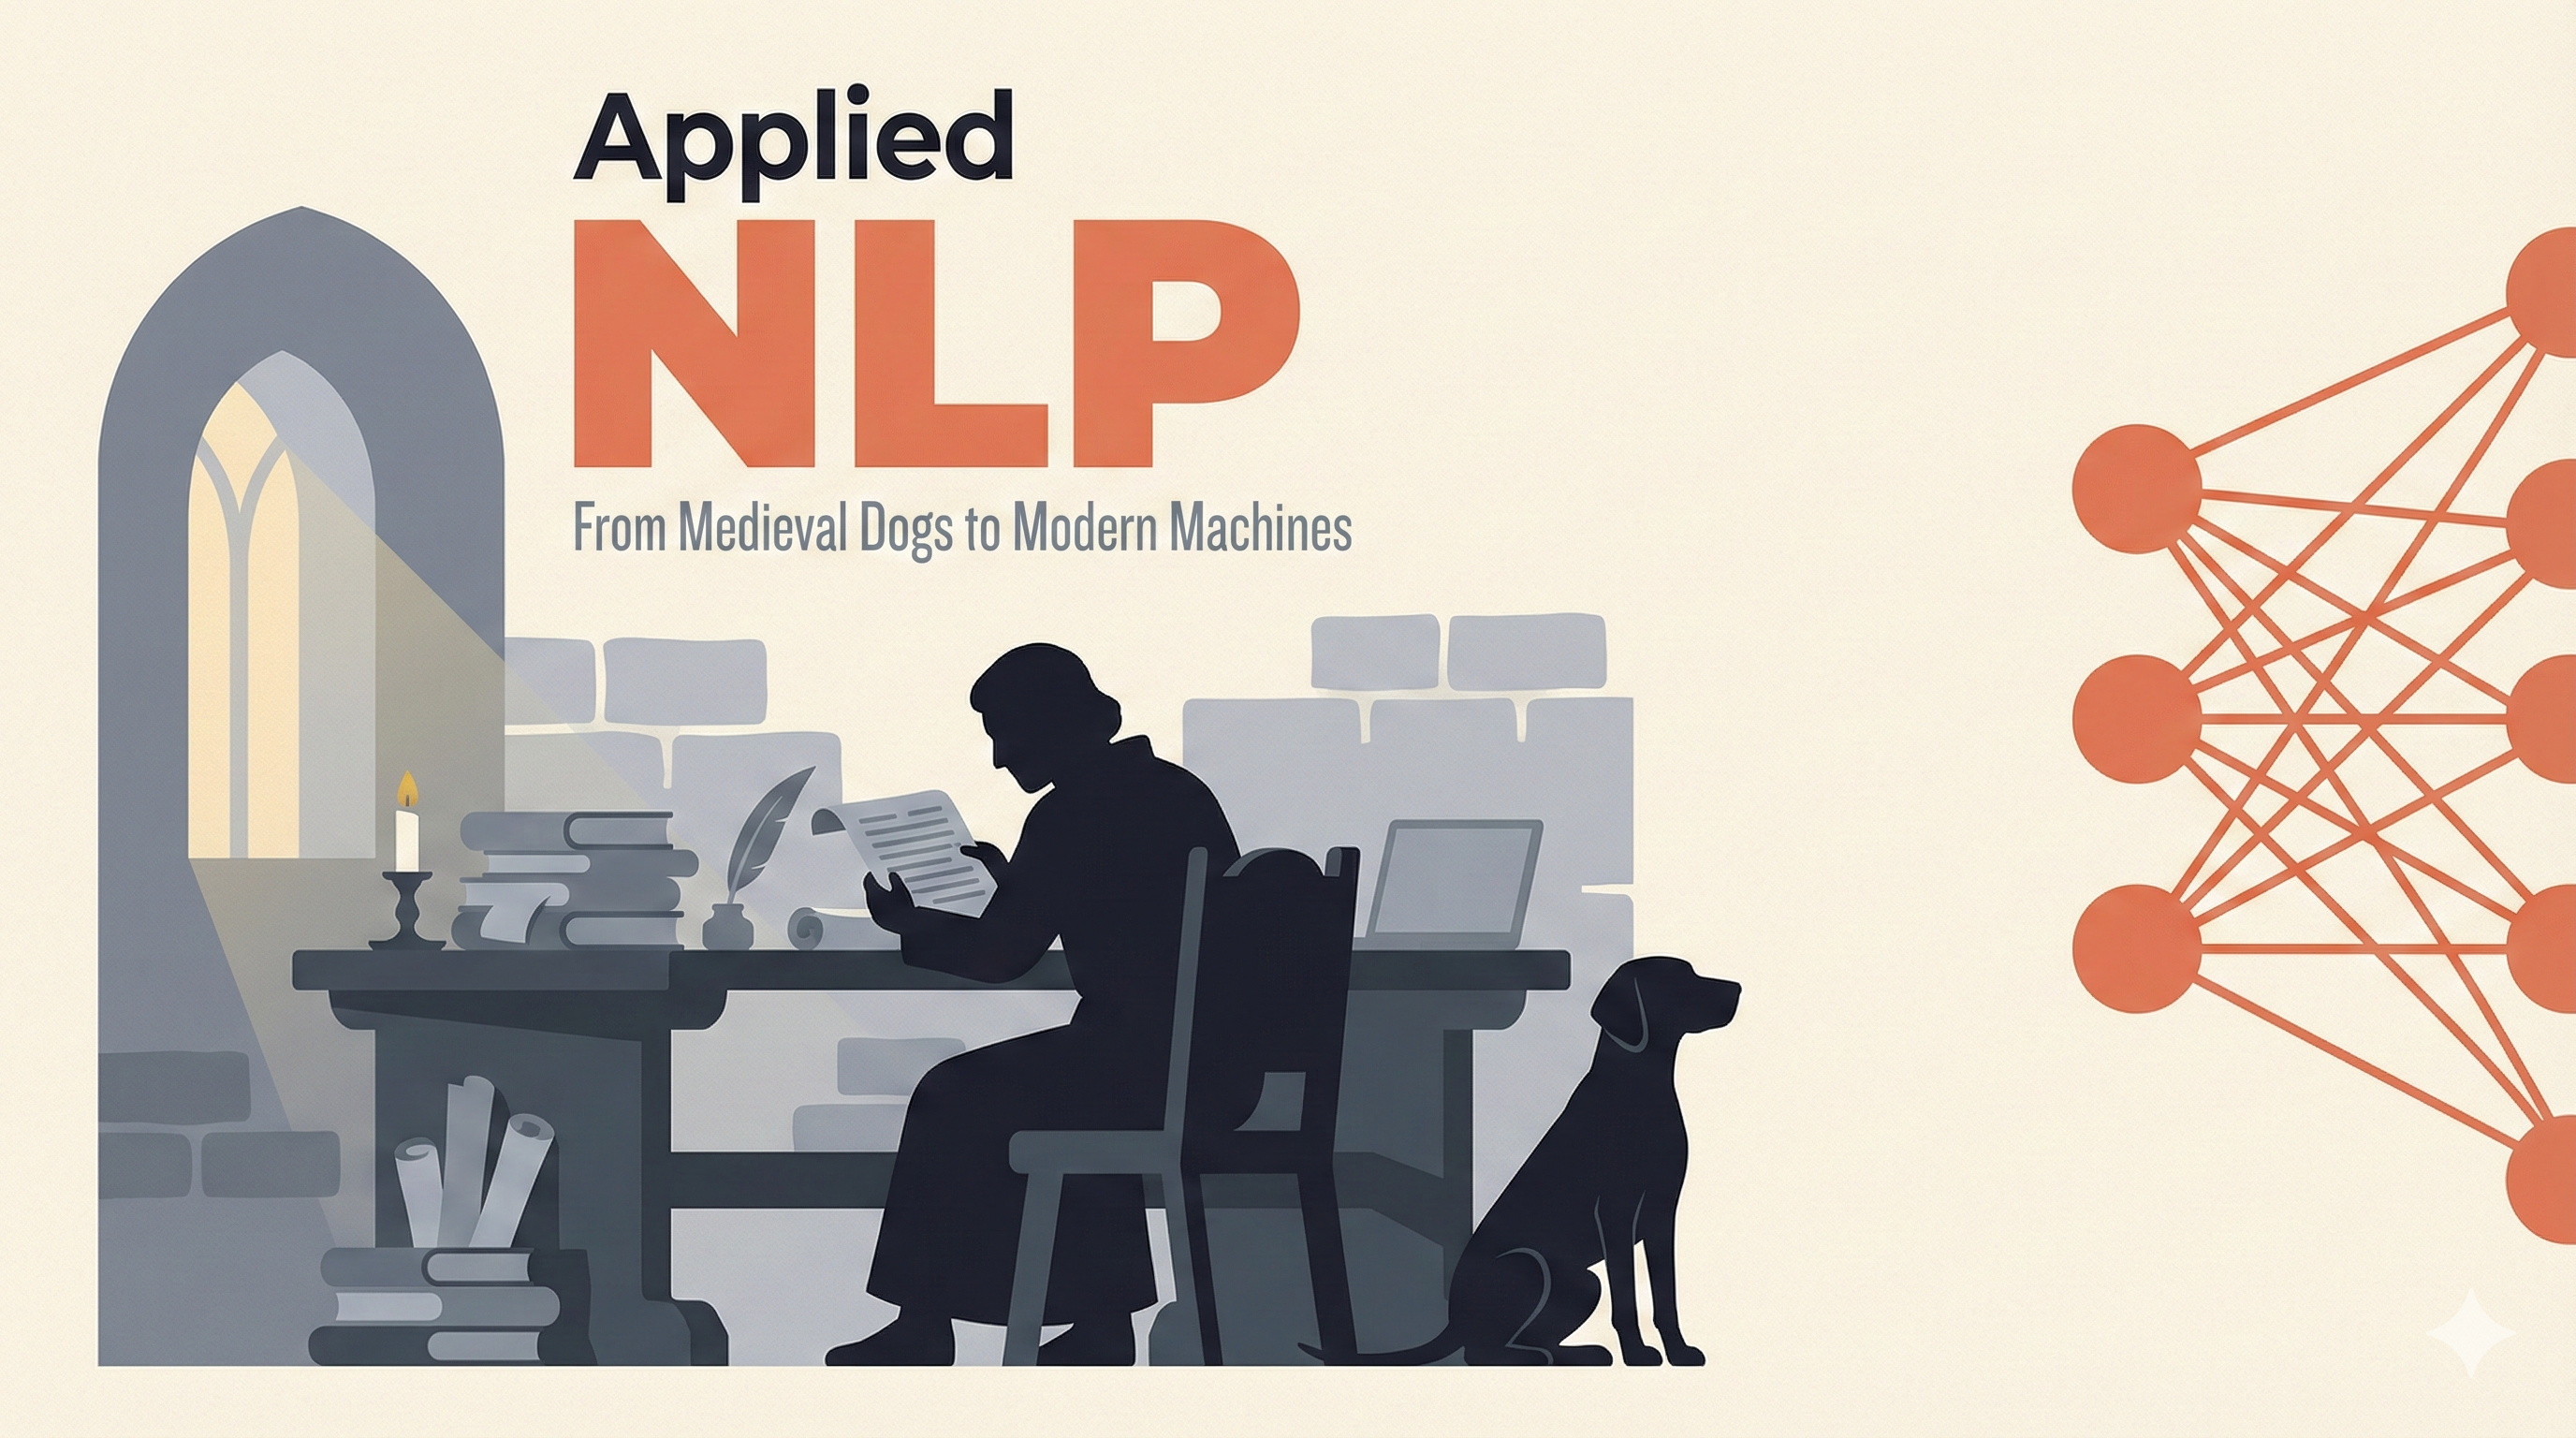
\includegraphics[width=\paperwidth,height=\paperheight,keepaspectratio]{figures/generated/title.png}
    \end{center}
  }{%
    \titlepage
  }
\end{frame}

% --- Slide 2: The Dual Track ---
\begin{frame}{Two Tracks}
  \framesubtitle{Concepts first, systems second}

  \begin{columns}[T]
    \begin{column}{0.47\textwidth}
      \highlight{Concepts \& Intuition}\\[0.2cm]
      We build mental models before code:\\[0.15cm]
      \begin{itemize}
        \item representation (counts $\to$ vectors $\to$ context)
        \item matching and retrieval (what is relevant?)
        \item structure (how we turn text into analyzable data)
      \end{itemize}
      \muted{Goal: understand why each method works and fails.}
    \end{column}
    \begin{column}{0.47\textwidth}
      \highlight{Operations on Text}\\[0.2cm]
      Treat text as a universal interface\\
      to documents, code, logs, and speech transcripts.\\[0.15cm]
      \gold{Classify} $\to$ assign labels\\
      \gold{Extract} $\to$ schema/JSON fields\\
      \gold{Retrieve} $\to$ evidence at scale\\
      \gold{Reason} $\to$ synthesize + decide\\[0.15cm]
      \muted{We move from simple pipelines to advanced systems.}
    \end{column}
  \end{columns}
\end{frame}

% --- Slide 3: Roadmap ---
\begin{frame}{Roadmap}
  \framesubtitle{Methods evolve, and so do capabilities}

  \begin{center}
  \begin{tikzpicture}[
    era/.style={rectangle, draw=coral, fill=bgcard, text=textdark, minimum width=1.8cm, minimum height=0.7cm, font=\footnotesize\bfseries, line width=0.5pt, align=center},
    year/.style={font=\tiny, text=gold},
    desc/.style={font=\scriptsize, text=textsecond, text width=1.8cm, align=center}
  ]
    \draw[coral, line width=1.5pt] (0,0) -- (14,0);
    \foreach \x/\yr/\name/\detail in {
      0.8/1990s/TF-IDF/Sparse weighting,
      3.2/2003/Topics/Latent structure,
      5.6/2013/Word2Vec/Dense semantics,
      8.0/2017/Transformers/Contextualization,
      10.4/2022+/LLMs/General text ops,
      12.8/2026/State of Art/Production workflows
    } {
      \fill[coral] (\x, 0) circle (3pt);
      \node[era, above=0.5cm] at (\x, 0) {\name};
      \node[year, below=0.15cm] at (\x, 0) {\yr};
      \node[desc, below=0.55cm] at (\x, 0) {\detail};
    }
  \end{tikzpicture}
  \end{center}

  \vspace{0.2cm}
  \begin{columns}[T]
    \begin{column}{0.48\textwidth}
      \highlight{Capability unlocks}
      \begin{itemize}
        \item Better representation of meaning
        \item Better handling of context and ambiguity
      \end{itemize}
    \end{column}
    \begin{column}{0.48\textwidth}
      \highlight{What scales now}
      \begin{itemize}
        \item extraction + labeling + retrieval at corpus scale
        \item hybrid workflows (classical + neural + LLM)
      \end{itemize}
    \end{column}
  \end{columns}

  \vspace{0.1cm}
  \muted{Each era adds tools; good systems combine them rather than replacing everything.}
\nobreak\cmark{Deerwester (1990); Blei (2003); Mikolov (2013); Vaswani (2017)}
\end{frame}


% ═══════════════════════════════════════════════════════════════
\section{TF-IDF \& Text Features}
% ═══════════════════════════════════════════════════════════════

% --- Slide 4: Word Counts ---
\begin{frame}{Word Counts \& Information Theory}
  \framesubtitle{The foundation of text retrieval}

  \begin{itemize}
    \item Text is \highlight{unstructured} --- the hardest data type for machines
    \item First idea: just \textbf{count words}
    \item Problem: common words (``the'', ``is'', ``and'') dominate
    \item Solution: weight words by how \highlight{informative} they are
  \end{itemize}

  \vspace{0.4cm}
  \begin{alertblock}{Information-Theory Lens}
    Self-information is \highlight{$I(x) = -\log p(x)$}: rare events carry more bits.\\
    IDF is mathematically equivalent to \highlight{self-information (surprisal)}.\\
    In text: rarer terms are often more discriminative.
  \end{alertblock}

  \cmark{Shannon, 1948; Sparck Jones, 1972; Aizawa, 2003}
\end{frame}

% --- Slide 5: Bag of Words ---
\begin{frame}{Bag of Words}
  \framesubtitle{The simplest text representation}

  \begin{center}
  \footnotesize
  \begin{tabular}{l|cccccc}
    \toprule
    & climate & tax & merger & trial & chatbot & patent \\
    \midrule
    \textit{``Climate patent trial update''} & \highlight{1} & 0 & 0 & \highlight{1} & 0 & \highlight{1} \\
    \textit{``Tax merger debate''} & 0 & \highlight{1} & \highlight{1} & 0 & 0 & 0 \\
    \textit{``Chatbot climate memo''} & \highlight{1} & 0 & 0 & 0 & \highlight{1} & 0 \\
    \bottomrule
  \end{tabular}
  \end{center}

  \vspace{0.4cm}
  \begin{itemize}
    \item Each document $=$ a vector of word frequencies
    \item \highlight{Ignores word order} (``dog bites man'' $=$ ``man bites dog'')
    \item But surprisingly effective for classification and retrieval
  \end{itemize}
\end{frame}

% --- Slide 6: TF-IDF Intuition ---
\begin{frame}{TF-IDF Intuition: Signal vs. Noise}
  \framesubtitle{What is distinctive in a noisy stream?}

  \begin{columns}[T]
    \begin{column}{0.48\textwidth}
      Imagine 100 AI company announcements this month.\\[0.25cm]
      \begin{itemize}
        \item Most repeat generic terms: \textbf{assistant}, \textbf{productivity}
        \item Those words are everywhere --- they barely distinguish documents
        \item One announcement includes \gold{clinical-trial evidence}
        \item That rare term is a strong pointer to a specific sub-topic
      \end{itemize}
      \vspace{0.2cm}
      \gold{TF-IDF} boosts words that are frequent \textit{in this document} but rare \textit{in the corpus}.
    \end{column}
    \begin{column}{0.49\textwidth}
      \begin{center}
        \begin{tikzpicture}[scale=0.96]
          \draw[textmuted, thin] (0,0) rectangle (6.2,4.8);
          \node[font=\small, text=textdark] at (3.1,5.1) {Document frequency in 100 docs};

          \node[font=\scriptsize, anchor=east, text=textsecond] at (1.25,4.0) {assistant};
          \fill[textmuted, opacity=0.35] (1.35,3.78) rectangle (5.5,4.18);
          \node[font=\scriptsize, anchor=west, text=textmuted] at (5.6,4.0) {80};

          \node[font=\scriptsize, anchor=east, text=textsecond] at (1.25,3.1) {productivity};
          \fill[textmuted, opacity=0.35] (1.35,2.88) rectangle (5.2,3.28);
          \node[font=\scriptsize, anchor=west, text=textmuted] at (5.3,3.1) {74};

          \node[font=\scriptsize, anchor=east, text=textsecond] at (1.25,2.2) {copilot};
          \fill[textmuted, opacity=0.35] (1.35,1.98) rectangle (4.9,2.38);
          \node[font=\scriptsize, anchor=west, text=textmuted] at (5.0,2.2) {68};

          \node[font=\scriptsize, anchor=east, text=gold] at (1.25,1.3) {clinical-trial};
          \fill[gold, opacity=0.9] (1.35,1.08) rectangle (1.7,1.48);
          \node[font=\scriptsize, anchor=west, text=gold] at (1.8,1.3) {2 (high IDF)};

          \node[font=\scriptsize, text=textmuted] at (3.1,0.4) {$\mathrm{IDF}(t)=\log\!\left(\frac{N}{\mathrm{df}(t)}\right)$};
        \end{tikzpicture}
      \end{center}
    \end{column}
  \end{columns}
\end{frame}

% --- Slide 7: TF-IDF Math ---
\begin{frame}{TF-IDF: The Math}

  \begin{center}
    {\Large $w(t, d) = \underbrace{\text{tf}(t, d)}_{\text{term frequency}} \times \underbrace{\log\!\left(\frac{N}{\text{df}(t)}\right)}_{\text{inverse document frequency}}$}
  \end{center}

  \vspace{0.3cm}
  \footnotesize
  \begin{center}
  \begin{tabular}{lcccl}
    \toprule
    \textbf{Term} & \textbf{TF in doc} & \textbf{DF (of 1000)} & \textbf{IDF} & \textbf{TF-IDF} \\
    \midrule
    ``assistant'' & 10/100 & 980 & $\log(1.02) \approx 0.02$ & 0.002 \\
    ``productivity'' & 7/100 & 720 & $\log(1.39) \approx 0.33$ & 0.023 \\
    ``clinical'' & 3/100 & 35 & $\log(28.6) \approx 3.35$ & \gold{0.101} \\
    ``oncology'' & 2/100 & 8 & $\log(125) \approx 4.83$ & \gold{0.097} \\
    \bottomrule
  \end{tabular}
  \end{center}

  \vspace{0.2cm}
  \muted{Common terms get low weight; domain-specific rare terms dominate TF-IDF signal.}
\end{frame}

% --- Slide 8: TF-IDF Worked Example ---
\begin{frame}{TF-IDF: A Worked Example}
  \framesubtitle{Numerical intuition with one announcement}

  \footnotesize
  Suppose one document has 80 tokens and discusses a clinical AI launch.

  \vspace{0.2cm}
  \begin{center}
  \begin{tabular}{lccccp{4.2cm}}
    \toprule
    \textbf{Term} & \textbf{TF} & \textbf{DF/1000} & \textbf{IDF} & \textbf{TF-IDF} & \textbf{Interpretation} \\
    \midrule
    assistant & $8/80$ & 950 & 0.05 & 0.005 & very common term, weak signal \\
    productivity & $5/80$ & 700 & 0.36 & 0.023 & moderately informative \\
    clinical & $3/80$ & 35 & 3.35 & \gold{0.126} & rare and highly distinctive \\
    oncology & $2/80$ & 8 & 4.83 & \gold{0.121} & very rare, high signal \\
    \bottomrule
  \end{tabular}
  \end{center}

  \vspace{0.2cm}
  \muted{Key idea: a term can appear fewer times but still dominate if it is globally rare.}
\end{frame}

% --- Slide 9: BM25 ---
\begin{frame}{BM25: TF-IDF's Descendant (Still Alive in 2026)}
  \framesubtitle{The algorithm that powers search engines}

  \begin{itemize}
    \item \highlight{BM25} adds \textbf{term frequency saturation}: $\frac{\text{tf}}{\text{tf} + k_1}$
    \item Prevents long documents from dominating
    \item Default in \textbf{Elasticsearch}, Apache Solr, Apache Lucene
  \end{itemize}

  \vspace{0.3cm}
  \begin{exampleblock}{2024: BMX --- The Next Step}
    BMX combines entropy-weighted similarity with TF-IDF.\\
    Outperforms BM25 on the BEIR benchmark.\\
    \muted{See Li et al., 2024 (arXiv:2408.06643).}
  \end{exampleblock}

  \vspace{0.3cm}
  \begin{center}
    \gold{Lesson:} foundational methods don't die --- they \highlight{evolve}.\\
    \muted{Every modern search engine still uses TF-IDF descendants.}
  \end{center}
\nobreak\cmark{Robertson et al., 1994; Robertson \& Zaragoza, 2009; Li et al., 2024}
\end{frame}


% ═══════════════════════════════════════════════════════════════
\section{Topic Modeling}
% ═══════════════════════════════════════════════════════════════

% --- Slide 10: Uncovering Hidden Relationships ---
\begin{frame}{Uncovering Hidden Relationships}
  \framesubtitle{From words to latent structure}

  \begin{columns}[T]
    \begin{column}{0.32\textwidth}
      \begin{block}{LSA / LSI}
        \tiny
        SVD on term-document matrix.\\
        Captures global co-occurrence.\\
        \muted{Deerwester et al., 1990}
      \end{block}
    \end{column}
    \begin{column}{0.32\textwidth}
      \begin{block}{LDA}
        \tiny
        Probabilistic generative model.\\
        Documents as topic mixtures.\\
        \muted{Blei et al., 2003}
      \end{block}
    \end{column}
    \begin{column}{0.32\textwidth}
      \begin{block}{NMF}
        \tiny
        Non-negative factorization.\\
        Usually easier to interpret.\\
        \muted{Lee \& Seung, 1999}
      \end{block}
    \end{column}
  \end{columns}

  \vspace{0.15cm}
  \small
  \begin{itemize}
    \item \highlight{Method evolution:} algebraic compression $\rightarrow$ probabilistic semantics $\rightarrow$ interpretable factorization.
    \item \highlight{In social science:} LDA became a workhorse, but evaluation remains partly subjective.
    \item Practical rule: judge quality by coherence, usefulness for the question, and human interpretability.
  \end{itemize}
\nobreak\cmark{Deerwester et al., 1990; Blei et al., 2003; Lee \& Seung, 1999}
\end{frame}

% --- Slide 11: Matrix Factorization (decomposition) ---
\begin{frame}{Matrix Factorization}
  \framesubtitle{Decomposing documents into hidden topics}

  \begin{center}
  \footnotesize
  $\underbrace{%
  \begin{pmatrix}
    3 & 0 & 2 & 0 & 1 \\
    0 & 2 & 0 & 3 & 0 \\
    2 & 0 & 3 & 0 & 1 \\
    0 & 1 & 0 & 2 & 0
  \end{pmatrix}}_{\textbf{A}\;\text{\tiny docs} \times \text{\tiny words}}
  \;\;\approx\;\;
  \underbrace{%
  \begin{pmatrix}
    \color{coral}0.9 & \color{gold}0.1 \\
    \color{coral}0.1 & \color{gold}0.9 \\
    \color{coral}0.8 & \color{gold}0.2 \\
    \color{coral}0.2 & \color{gold}0.8
  \end{pmatrix}}_{\textbf{W}\;\text{\tiny docs} \times \text{\tiny\color{coral}topics}}
  \;\times\;
  \underbrace{%
  \begin{pmatrix}
    \color{coral}3.2 & \color{coral}0.0 & \color{coral}2.5 & \color{coral}0.1 & \color{coral}1.0 \\
    \color{gold}0.1 & \color{gold}2.0 & \color{gold}0.0 & \color{gold}2.8 & \color{gold}0.0
  \end{pmatrix}}_{\textbf{H}\;\text{\tiny\color{gold}topics} \times \text{\tiny words}}$
  \end{center}

  \vspace{0.4cm}
  \begin{columns}[T]
    \begin{column}{0.48\textwidth}
      \highlight{Column labels for A and H:}\\[0.1cm]
      \muted{\footnotesize inflation, patent, rates, startup, fiscal}
    \end{column}
    \begin{column}{0.48\textwidth}
      \highlight{Two topics emerge:}\\[0.1cm]
      \muted{\footnotesize \textcolor{coral}{Topic A}: inflation, rates, fiscal}\\
      \muted{\footnotesize \textcolor{gold}{Topic B}: patent, startup}
    \end{column}
  \end{columns}
\end{frame}

% --- Slide 11b: Matrix Factorization (interpretation) ---
\begin{frame}{Matrix Factorization: Reading the Result}
  \framesubtitle{What \textbf{W} and \textbf{H} tell us}

  \begin{columns}[T]
    \begin{column}{0.48\textwidth}
      \highlight{\textbf{W}: document--topic mixtures}\\[0.2cm]
      \footnotesize
      \begin{tabular}{lcc}
        \toprule
        & \textcolor{coral}{Econ} & \textcolor{gold}{Tech} \\
        \midrule
        Doc 1 & \textcolor{coral}{\textbf{0.9}} & \textcolor{gold}{0.1} \\
        Doc 2 & \textcolor{coral}{0.1} & \textcolor{gold}{\textbf{0.9}} \\
        Doc 3 & \textcolor{coral}{\textbf{0.8}} & \textcolor{gold}{0.2} \\
        Doc 4 & \textcolor{coral}{0.2} & \textcolor{gold}{\textbf{0.8}} \\
        \bottomrule
      \end{tabular}\\[0.2cm]
      \muted{Docs 1 \& 3 are mostly economics.\\Docs 2 \& 4 are mostly tech.}
    \end{column}
    \begin{column}{0.48\textwidth}
      \highlight{\textbf{H}: topic--word distributions}\\[0.2cm]
      \footnotesize
      \begin{tabular}{lccccc}
        \toprule
        & \rotatebox{50}{\tiny inflation} & \rotatebox{50}{\tiny patent} & \rotatebox{50}{\tiny rates} & \rotatebox{50}{\tiny startup} & \rotatebox{50}{\tiny fiscal} \\
        \midrule
        \textcolor{coral}{Econ} & \textcolor{coral}{\textbf{3.2}} & 0.0 & \textcolor{coral}{\textbf{2.5}} & 0.1 & \textcolor{coral}{\textbf{1.0}} \\
        \textcolor{gold}{Tech} & 0.1 & \textcolor{gold}{\textbf{2.0}} & 0.0 & \textcolor{gold}{\textbf{2.8}} & 0.0 \\
        \bottomrule
      \end{tabular}\\[0.2cm]
      \muted{Each topic has a distinct\\word signature.}
    \end{column}
  \end{columns}

  \vspace{0.3cm}
  \begin{center}
    We choose $k$ topics --- the model finds the \gold{best decomposition}.\\
    \muted{NMF: non-negative values only. LDA: probabilistic (Dirichlet priors).}
  \end{center}

  \cmark{Deerwester et al., 1990; Lee \& Seung, 1999}
\end{frame}

% --- Slide 11b: Topic Model Visualization (generated asset) ---
\begin{frame}[plain]
  \IfFileExists{figures/generated/topic_model_viz.png}{%
    \hspace*{-0.8cm}%
    \includegraphics[width=0.95\paperwidth,height=0.95\paperheight,keepaspectratio]{figures/generated/topic_model_viz.png}
  }{%
    \vspace*{0.12\paperheight}
    \begin{center}
      {\Large\textbf{Topic Model Visualization (Placeholder)}}\\[0.35cm]
      \setlength{\fboxsep}{12pt}
      \fcolorbox{coral}{bgcard}{%
        \parbox{0.82\paperwidth}{%
          \centering
          \small
          Awaiting generated full-slide image.\\[0.15cm]
          Add the rendered topic-model figure in the generated figures folder\\
          and recompile to replace this placeholder.
        }%
      }
    \end{center}
  }
\end{frame}

% --- Slide 12: Discovering Topics ---
\begin{frame}{Discovering Topics in Text}
  \framesubtitle{Automatic theme extraction from a large corpus}

  \small
  Feed 10,000 documents into a topic model $\rightarrow$ four coherent themes:

  \vspace{0.2cm}
  \begin{columns}[T]
    \begin{column}{0.48\textwidth}
      \begin{block}{Technology}
        \scriptsize AI, startup, funding, platform, compute, deploy
      \end{block}
      \begin{block}{Economics}
        \scriptsize inflation, GDP, labor, trade, policy, fiscal
      \end{block}
    \end{column}
    \begin{column}{0.48\textwidth}
      \begin{block}{Climate}
        \scriptsize emissions, carbon, renewable, ESG, transition, green
      \end{block}
      \begin{block}{Health}
        \scriptsize vaccine, trial, patients, drug, biotech, FDA
      \end{block}
    \end{column}
  \end{columns}

  \vspace{0.2cm}
  \begin{center}
    \muted{An article on ``AI for drug discovery'':}
    \highlight{50\%} Technology,
    \highlight{30\%} Health,
    \muted{20\% other}\\[0.1cm]
    \muted{Documents are mixtures, not single labels.}
  \end{center}
\end{frame}

% --- Slide 13: LDA ---
\begin{frame}{LDA: The Generative Model}
  \framesubtitle{Formal process + plain-language intuition}

  \begin{columns}[T]
    \begin{column}{0.5\textwidth}
      \small
      \textbf{Generative story}
      \begin{enumerate}
        \item Draw document topic mix: $\theta_d \sim \text{Dir}(\alpha)$
        \item For each token position $n$, sample a topic: $z_{d,n} \sim \text{Mult}(\theta_d)$
        \item Sample a word from that topic: $w_{d,n} \sim \text{Mult}(\phi_{z_{d,n}})$
      \end{enumerate}
      \muted{Intuition: pick a theme, then pick a word typical for that theme.}
    \end{column}
    \begin{column}{0.47\textwidth}
      \begin{center}
      \begin{tikzpicture}[scale=0.78]
        \node[circle, draw=gold, fill=bgcard, text=textdark, minimum size=0.8cm] (theta) at (0,0) {$\theta$};
        \node[circle, draw=coral, fill=bgcard, text=textdark, minimum size=0.8cm] (z) at (2.5,0) {$z$};
        \node[circle, draw=textsecond, fill=bgcard, text=textdark, minimum size=0.8cm] (w) at (5,0) {$w$};
        \node[circle, draw=gold, fill=bgcard, text=textdark, minimum size=0.8cm] (phi) at (2.5,1.5) {$\phi$};
        \draw[-{Stealth}, gold, thick] (theta) -- (z);
        \draw[-{Stealth}, coral, thick] (z) -- (w);
        \draw[-{Stealth}, gold, thick] (phi) -- (w);
        \node[font=\tiny, text=textmuted] at (0, -0.7) {topic mix};
        \node[font=\tiny, text=textmuted] at (2.5, -0.7) {topic};
        \node[font=\tiny, text=textmuted] at (5, -0.7) {word};
        \node[font=\tiny, text=textmuted] at (2.5, 2.1) {topic-word dist.};
      \end{tikzpicture}
      \end{center}

      \vspace{0.1cm}
      \scriptsize
      Example token flow:\\
      \texttt{[Topic=Health]} $\rightarrow$ \texttt{vaccine}\\
      \texttt{[Topic=Economics]} $\rightarrow$ \texttt{inflation}
    \end{column}
  \end{columns}

  \vspace{0.1cm}
  \cmark{Blei, Ng \& Jordan, 2003}
\end{frame}

% --- Slide 14: BERTopic ---
\begin{frame}{BERTopic: Topic Modeling for 2026}
  \framesubtitle{Embeddings + clustering + interpretability}

  \IfFileExists{figures/generated/bertopic.png}{%
    \begin{center}
      \includegraphics[width=0.94\textwidth]{figures/generated/bertopic.png}
    \end{center}
  }{%
    \begin{center}
    \begin{tikzpicture}[
      pipestep/.style={rectangle, draw=coral, fill=bgcard, text=textdark, minimum width=2.2cm, minimum height=1cm, font=\footnotesize, align=center, line width=0.5pt},
      arr/.style={-{Stealth}, coral, thick}
    ]
      \node[pipestep] (embed) at (0,0) {Embed\\[-0.05cm]\tiny sentence-transformers};
      \node[pipestep] (umap) at (3.5,0) {Reduce\\[-0.05cm]\tiny UMAP};
      \node[pipestep] (hdbscan) at (7,0) {Cluster\\[-0.05cm]\tiny HDBSCAN};
      \node[pipestep] (ctfidf) at (10.5,0) {Represent\\[-0.05cm]\tiny c-TF-IDF};
      \draw[arr] (embed) -- (umap);
      \draw[arr] (umap) -- (hdbscan);
      \draw[arr] (hdbscan) -- (ctfidf);
    \end{tikzpicture}
    \end{center}
  }

  \vspace{0.05cm}
  \footnotesize
  \begin{columns}[T]
    \begin{column}{0.48\textwidth}
      \highlight{Advantages over LDA:}
      \begin{itemize}\itemsep2pt
        \item Auto-selects topic count
        \item 50+ languages
        \item LLM-assisted topic labels
        \item Local models run on laptops (privacy + cost)
      \end{itemize}
    \end{column}
    \begin{column}{0.48\textwidth}
      \highlight{Benchmark:}
      \begin{itemize}\itemsep2pt
        \item Coherence (Cv): \gold{0.76} \muted{vs LDA 0.38 ($\sim$2$\times$)}
        \item Strong open-source ecosystem + notebook tooling
        \item New releases: multi-GPU and Model2Vec support
      \end{itemize}
    \end{column}
  \end{columns}

  \cmark{Grootendorst, 2022; arXiv:2203.05794}
\end{frame}

% --- Slide 15: BERTopic in Practice ---
\begin{frame}{BERTopic in Practice}
  \framesubtitle{Why social scientists love it}

  \begin{itemize}
    \item \highlight{Interpretable}: c-TF-IDF gives real words per topic (not just topic IDs)
    \item \highlight{Scalable}: handles 100K+ documents on a laptop
    \item \highlight{LLM integration}: feed topic words to GPT/Claude for human-readable names
    \item \highlight{Visualization}: built-in topic maps, hierarchies, temporal trends
    \item \highlight{Local-first option}: strong small/local models can label topics offline
  \end{itemize}

  \vspace{0.3cm}
  \begin{alertblock}{Bridge to Social Science}
    BERTopic is the most adopted topic model in social science since LDA.\\
    Used in: innovation studies, policy analysis, media research, scientometrics.
  \end{alertblock}

  \vspace{0.1cm}
  \muted{We'll build a full BERTopic pipeline in \highlight{NB04}, including a topic map and LLM topic naming.}
\end{frame}


% ═══════════════════════════════════════════════════════════════
\section{Word Embeddings \& Vector Space}
% ═══════════════════════════════════════════════════════════════

% --- Slide 16: Words as GPS Coordinates ---
\begin{frame}{Words as GPS Coordinates}
  \framesubtitle{From sparse counts to dense meaning}

  \begin{columns}[T]
    \begin{column}{0.55\textwidth}
      TF-IDF: each word = a dimension (10,000+ dims)\\[0.2cm]
      \highlight{Word2Vec}: each word = a \textbf{dense vector} (100--300 dims)\\[0.3cm]
      Think of it as \gold{GPS coordinates in meaning-space}:
      \begin{itemize}\itemsep2pt
        \item ``dog'' and ``puppy'' are \highlight{nearby}
        \item ``dog'' and ``spreadsheet'' are \highlight{far apart}
        \item Similar meanings $\to$ similar coordinates
      \end{itemize}
      \vspace{0.2cm}
      \muted{Distributional idea: ``you know a word by the company it keeps.'' Meaning emerges from context at scale.}
    \end{column}
    \begin{column}{0.4\textwidth}
      \begin{center}
      \begin{tikzpicture}[scale=0.7]
        \draw[textmuted, semithick, ->] (0,0) -- (5,0) node[right, font=\tiny, text=textmuted] {dim 1};
        \draw[textmuted, semithick, ->] (0,0) -- (0,5) node[above, font=\tiny, text=textmuted] {dim 2};
        % Animal cluster
        \fill[coral] (1.5,3.5) circle (3pt) node[right, font=\footnotesize, text=textdark] {dog};
        \fill[coral] (1.8,3.8) circle (3pt) node[right, font=\footnotesize, text=textdark] {puppy};
        \fill[corallight] (2.2,3.0) circle (3pt) node[right, font=\footnotesize, text=textsecond] {cat};
        \fill[corallight] (1.2,2.7) circle (3pt) node[left, font=\footnotesize, text=textsecond] {kitten};
        % Far away
        \fill[textmuted] (4.0,0.8) circle (3pt) node[right, font=\footnotesize, text=textmuted] {spreadsheet};
        \fill[textmuted] (3.8,1.2) circle (3pt) node[left, font=\footnotesize, text=textmuted] {excel};
        % Cluster labels
        \draw[coral, dashed, thick] (0.7,2.4) ellipse (1.5cm and 1.2cm);
        \draw[textmuted, dashed] (3.5,0.6) ellipse (1.2cm and 0.8cm);
      \end{tikzpicture}
      \end{center}
    \end{column}
  \end{columns}

  \cmark{Mikolov et al., 2013}
\end{frame}

% --- Slide 17: King - Man + Woman = Queen ---
\begin{frame}{Vector Arithmetic}
  \framesubtitle{The most famous equation in NLP}

  \begin{center}
    {\Large\color{gold} $\vec{\text{king}} - \vec{\text{man}} + \vec{\text{woman}} \approx \vec{\text{queen}}$}
  \end{center}

  \vspace{0.4cm}
  \begin{center}
  \begin{tikzpicture}[scale=0.82]
    \node[font=\normalsize, text=textdark] (king) at (0.4,3.0) {\textbf{king}};
    \node[font=\normalsize, text=textdark] (queen) at (4.6,2.5) {\textbf{queen}};
    \node[font=\normalsize, text=textdark] (man) at (0.0,0.0) {\textbf{man}};
    \node[font=\normalsize, text=textdark] (woman) at (4.2,-0.5) {\textbf{woman}};
    \draw[-{Stealth}, coral, thick] (man) -- (king) node[midway, left, font=\footnotesize, text=gold] {royalty};
    \draw[-{Stealth}, coral, thick] (woman) -- (queen) node[midway, right, font=\footnotesize, text=gold] {royalty};
    \draw[-{Stealth}, textmuted, thick] (man) -- (woman) node[midway, below, font=\footnotesize, text=textmuted] {gender};
    \draw[-{Stealth}, textmuted, thick] (king) -- (queen) node[midway, above, font=\footnotesize, text=textmuted] {gender};
  \end{tikzpicture}
  \end{center}

  \vspace{0.3cm}
  \begin{center}
    \muted{Works for:} \gold{Paris} $-$ \gold{France} $+$ \gold{Germany} $\approx$ \gold{Berlin}\\
    \muted{Captures relational structure, not just similarity.}
  \end{center}
\end{frame}

% --- Slide 18: Training ---
\begin{frame}{How Word2Vec Learns}
  \framesubtitle{Predicting context from massive text corpora}

  The model reads thousands of books, predicting words from context:

  \vspace{0.2cm}
  \begin{center}
    \muted{``The} \highlight{dog} \muted{fetched the} \gold{[\_\_\_\_\_]} \muted{from the garden.''}
  \end{center}

  \vspace{0.3cm}
  \begin{center}
  \begin{tikzpicture}[scale=0.85]
    % Sliding window
    \foreach \i/\word in {0/The, 1.5/quick, 3/brown, 4.5/fox, 6/jumps} {
      \node[font=\small, text=textdark] at (\i, 0) {\word};
    }
    % Window highlight
    \draw[coral, thick, rounded corners=3pt] (0.6,-0.3) rectangle (5.4,0.4);
    \node[font=\tiny, text=coral] at (3,0.7) {context window};
    % Arrows
    \draw[-{Stealth}, gold, thick] (1.5,-0.5) -- (3,-1.2);
    \draw[-{Stealth}, gold, thick] (4.5,-0.5) -- (3,-1.2);
    \node[font=\small, text=gold] at (3,-1.5) {predict ``brown''};
  \end{tikzpicture}
  \end{center}

  \vspace{0.2cm}
  \begin{itemize}
    \item \textbf{Skip-gram}: predict context from center word
    \item \textbf{CBOW}: predict center word from context
    \item Words that appear in similar contexts get \highlight{similar vectors}
  \end{itemize}

  \cmark{Mikolov et al., 2013; Pennington et al. (GloVe), 2014}
\end{frame}

% --- Slide 18b: Full-Screen UFO in the Village ---
\begin{frame}[plain]
  \begin{tikzpicture}[remember picture, overlay]
    \fill[bglight] (current page.south west) rectangle (current page.north east);
    % Axes
    \draw[textmuted, thin, ->] ([shift={(1.5cm,1.2cm)}]current page.south west) -- ([shift={(15cm,1.2cm)}]current page.south west);
    \draw[textmuted, thin, ->] ([shift={(1.5cm,1.2cm)}]current page.south west) -- ([shift={(1.5cm,8.5cm)}]current page.south west);
    % Medieval village cluster (large, left-center)
    \fill[gold] (4.5,5.5) circle (7pt) node[above=4pt, font=\normalsize, text=gold] {\textbf{castle}};
    \fill[gold] (5.3,4.6) circle (7pt) node[right=4pt, font=\normalsize, text=gold] {\textbf{knight}};
    \fill[gold] (3.5,4.2) circle (7pt) node[left=4pt, font=\normalsize, text=gold] {\textbf{sword}};
    \fill[gold] (4.0,3.5) circle (6pt) node[left=4pt, font=\small, text=gold] {armor};
    \fill[gold] (5.8,5.2) circle (6pt) node[right=4pt, font=\small, text=gold] {moat};
    \fill[coral] (6.2,4.0) circle (7pt) node[right=4pt, font=\normalsize, text=coral] {\textbf{dog}};
    \fill[coral] (6.8,4.8) circle (6pt) node[right=4pt, font=\small, text=coral] {hound};
    \fill[coral] (3.8,5.0) circle (5pt) node[left=4pt, font=\small, text=coral] {horse};
    \draw[gold, dashed, thick, rounded corners=10pt] (3.0,3.0) rectangle (7.3,6.0);
    \node[font=\small, text=textmuted] at (5.1,2.6) {medieval cluster};
    % UFO cluster (far right, isolated)
    \fill[textdark] (12.5,3.0) circle (9pt);
    \node[font=\Large\bfseries, text=textdark] at (12.5,3.8) {UFO};
    \fill[textmuted] (13.3,2.2) circle (6pt) node[right=3pt, font=\normalsize, text=textmuted] {spaceship};
    \fill[textmuted] (11.8,2.0) circle (6pt) node[left=3pt, font=\normalsize, text=textmuted] {alien};
    \fill[textmuted] (12.8,1.5) circle (5pt) node[right=3pt, font=\small, text=textmuted] {laser};
    \draw[textmuted, dashed, thick, rounded corners=8pt] (11.2,1.0) rectangle (14.0,3.5);
    % Distance arrow
    \draw[coral, thick, <->, line width=1.5pt] (7.5,4.5) -- (11.0,3.2);
    \node[font=\normalsize\bfseries, text=coral, rotate=-18] at (9.2,4.3) {large distance = dissimilarity};
    % Title
    \node[font=\Large\bfseries, text=textdark] at (8,8) {The UFO in the Village};
    \node[font=\normalsize, text=textmuted] at (8,7.4) {Concepts that never co-occur end up far apart in vector space.};
  \end{tikzpicture}
\end{frame}

% --- Slide 19: The UFO in the Village ---
\begin{frame}{The UFO in the Village}
  \framesubtitle{Distance = dissimilarity in vector space}

  \begin{columns}[T]
    \begin{column}{0.42\textwidth}
      \begin{itemize}
        \item Frequent co-occurrence pulls vectors together.
        \item Rare concepts with different context drift far away.
        \item Distance in embedding space approximates semantic distance.
      \end{itemize}
      \vspace{0.15cm}
      \muted{Distributional hypothesis: ``You shall know a word by the company it keeps.''}
      \vspace{0.1cm}
      \muted{If ``UFO'' rarely appears with village-life terms, it lands in a different region.}
    \end{column}
    \begin{column}{0.54\textwidth}
      \begin{center}
      \begin{tikzpicture}[scale=0.82]
        \draw[textmuted, thin, ->] (0,0) -- (7.2,0) node[right, font=\tiny, text=textmuted] {dim 1};
        \draw[textmuted, thin, ->] (0,0) -- (0,5.3) node[above, font=\tiny, text=textmuted] {dim 2};
        % Village cluster
        \fill[coral] (1.3,1.2) circle (3pt) node[left, font=\scriptsize, text=textdark] {castle};
        \fill[coral] (2.0,1.6) circle (3pt) node[above, font=\scriptsize, text=textdark] {knight};
        \fill[corallight] (2.4,0.95) circle (3pt) node[right, font=\scriptsize, text=textsecond] {sword};
        \fill[corallight] (1.8,0.65) circle (3pt) node[below, font=\scriptsize, text=textsecond] {village};
        \draw[coral, dashed, thick] (1.9,1.1) ellipse (1.45cm and 0.9cm);
        \node[font=\tiny, text=coral] at (1.9,2.15) {village semantics};

        % UFO cluster
        \fill[blue] (5.8,4.2) circle (3pt) node[right, font=\scriptsize, text=textdark] {UFO};
        \fill[blue] (5.2,3.75) circle (3pt) node[left, font=\scriptsize, text=textdark] {alien};
        \draw[blue, dashed, thick] (5.5,4.0) ellipse (0.95cm and 0.7cm);
        \node[font=\tiny, text=blue] at (5.55,4.95) {alien context};

        % Distance cue
        \draw[-{Stealth}, gold, thick] (3.0,2.0) -- (4.6,3.4);
        \node[font=\tiny, text=textdark, rotate=35] at (3.8,2.75) {large vector distance};
      \end{tikzpicture}
      \end{center}

    \end{column}
  \end{columns}
\end{frame}

% --- Slide 20: Visualizing Embeddings ---
\begin{frame}{Visualizing Embedding Space}
  \framesubtitle{From 300 dimensions down to 2 --- PCA vs.\ t-SNE vs.\ UMAP on real data}

  \begin{center}
    \includegraphics[width=0.92\textwidth]{figures/gemini/dim_reduc_PBMC_3k_example.png}
  \end{center}

  \vspace{0.1cm}
  \footnotesize
  \begin{columns}[T]
    \begin{column}{0.32\textwidth}
      \centering
      \highlight{PCA}\\
      \muted{Linear. Preserves global\\variance. Clusters overlap.}
    \end{column}
    \begin{column}{0.32\textwidth}
      \centering
      \highlight{t-SNE}\\
      \muted{Non-linear. Preserves local\\neighborhoods. Tight clusters.}
    \end{column}
    \begin{column}{0.32\textwidth}
      \centering
      \highlight{UMAP}\\
      \muted{Non-linear. Preserves both\\local + global structure.}
    \end{column}
  \end{columns}

  \vspace{0.1cm}
  \begin{center}
    \muted{PBMC 3K dataset: 3,000 blood cells, 5 cell types. Same embeddings, different projections.}
  \end{center}
\end{frame}

% --- Slide 21: Bias in Embeddings ---
\begin{frame}{Bias in Embeddings}
  \framesubtitle{A warning for social scientists}

  \begin{itemize}
    \item Word2Vec trained on Google News:
      \begin{itemize}
        \item ``man'' $\to$ ``computer programmer''
        \item ``woman'' $\to$ ``homemaker''
      \end{itemize}
    \item Embeddings \highlight{absorb and amplify} societal biases from training data
    \item WEAT test: measures stereotypes in embedding space
  \end{itemize}

  \vspace{0.3cm}
  \begin{alertblock}{For Social Scientists}
    This is both a \textbf{bug} and a \textbf{feature}:\\
    --- Bug: biased models produce biased outputs\\
    --- Feature: embeddings \highlight{measure cultural associations} at scale
  \end{alertblock}

  \cmark{Bolukbasi et al., 2016; Caliskan et al., 2017; Kozlowski et al., 2019}
\end{frame}

% --- Slide 22: Sentence Embeddings ---
\begin{frame}{From Words to Sentences}
  \framesubtitle{Sentence-BERT and the MTEB era}

  \begin{columns}[T]
    \begin{column}{0.48\textwidth}
      \begin{itemize}
        \item Word2Vec: one vector per \textit{word}
        \item \highlight{Sentence-BERT}: one vector per sentence/paragraph
        \item \textbf{MTEB} = Massive Text Embedding Benchmark
        \item Multilingual embeddings map similar meaning across languages into nearby regions
      \end{itemize}
      \vspace{0.15cm}
      \muted{Practical speedup: pairwise semantic search drops from hours to seconds with bi-encoder embeddings.}
    \end{column}
    \begin{column}{0.48\textwidth}
      \highlight{Provider landscape:}
      \begin{itemize}
        \item API: OpenAI, Gemini, xAI/Grok (where available)
        \item Local/open: SBERT, BGE, E5, LLM-derived embeddings
        \item Ollama + HF pipelines for local-first workflows
      \end{itemize}
      \vspace{0.12cm}
      \highlight{Ops tips:}
      \begin{itemize}
        \item Batch embedding APIs for cost/performance
        \item Cache vectors and version your embedding model
      \end{itemize}
    \end{column}
  \end{columns}

  \cmark{Reimers \& Gurevych, 2019}
\end{frame}


% ═══════════════════════════════════════════════════════════════
\section{Transformers}
% ═══════════════════════════════════════════════════════════════

% --- Slide 23: Attention Is All You Need ---
\begin{frame}{Attention Is All You Need}
  \framesubtitle{The paper that changed everything (Vaswani et al., 2017)}

  \highlight{Self-attention}: every word looks at every other word simultaneously.\\[0.3cm]

  \begin{columns}[T]
    \begin{column}{0.48\textwidth}
      \highlight{Why attention was needed:}
      \begin{itemize}\itemsep2pt
        \item RNNs process words one-by-one (slow, lossy)
        \item Attention processes \textit{all at once} (parallel)
        \item Long-range dependencies captured directly
        \item Enabled scaling to billions of parameters
      \end{itemize}
    \end{column}
    \begin{column}{0.48\textwidth}
      \highlight{Self-attention via Q/K/V:}\\[0.1cm]
      \begin{itemize}\itemsep2pt
        \item \textbf{Query}: what am I looking for?
        \item \textbf{Key}: what do I contain?
        \item \textbf{Value}: what do I offer?
      \end{itemize}
      \vspace{0.2cm}
      \muted{Analogy: Query = your search text,\\
      Key = the page title,\\
      Value = the page content}
    \end{column}
  \end{columns}

  \vspace{0.2cm}
  \cmark{Vaswani et al., 2017}
\end{frame}

% --- Slide 23-img: Attention Visualization (full slide) ---
\begin{frame}{Attention in Action}
  \framesubtitle{How the mechanism actually works}

  \begin{center}
    \IfFileExists{figures/generated/attention.png}{%
      \includegraphics[width=0.85\textwidth,height=0.75\textheight,keepaspectratio]{figures/generated/attention.png}
    }{%
      \IfFileExists{figures/gemini/attention.png}{%
        \includegraphics[width=0.85\textwidth,height=0.75\textheight,keepaspectratio]{figures/gemini/attention.png}
      }{%
        \fcolorbox{coral}{bgcard}{\parbox{0.8\textwidth}{\centering\small Missing image: \texttt{figures/generated/attention.png} or \texttt{figures/gemini/attention.png}}}
      }
    }
  \end{center}

  \vspace{0.1cm}
  \begin{center}
    \muted{Each token attends to every other token. Line thickness = attention weight.\\
    The model learns \textit{which} words matter for each word.}
  \end{center}
\end{frame}

% --- Slide 23b removed: feedback said viz doesn't work, replaced by full-slide image above ---

% --- Slide 24: The Assembly Line ---
\begin{frame}{The Assembly Line Analogy}
  \framesubtitle{Each transformer layer adds context --- like stations on a production line}

  \begin{center}
  \begin{tikzpicture}[
    layer/.style={rectangle, draw=coral, fill=bgcard, text=textdark, minimum width=10cm, minimum height=0.7cm, font=\footnotesize, line width=0.5pt},
  ]
    \node[layer] (l1) at (0,0) {Layer 1: ``king'' $\to$ a male ruler};
    \node[layer] (l2) at (0,1.2) {Layer 2: $\to$ a \textbf{Scottish} male ruler};
    \node[layer] (l3) at (0,2.4) {Layer 3: $\to$ who \textbf{murdered} the previous king};
    \node[layer] (l4) at (0,3.6) {Layer 4: $\to$ described in \textbf{Shakespearean} language};
    \draw[-{Stealth}, coral, thick] (0,-0.5) -- (0,-0.1);
    \draw[-{Stealth}, coral, thick] (l1.north) -- (l2.south);
    \draw[-{Stealth}, coral, thick] (l2.north) -- (l3.south);
    \draw[-{Stealth}, coral, thick] (l3.north) -- (l4.south);
    \node[font=\small, text=gold] at (0,-0.8) {raw token: ``king''};
    \node[font=\small, text=gold] at (0,4.2) {rich contextual representation};
  \end{tikzpicture}
  \end{center}

  \vspace{0.2cm}
  \muted{Like an assembly line: each station adds detail. The final product is\\a rich, context-aware representation --- ``king'' in \textit{Macbeth} $\neq$ ``king'' in a chess manual.}
\end{frame}

% --- Slide 25: Three Architectures ---
\begin{frame}{Three Transformer Architectures}

  \begin{center}
  \footnotesize
  \begin{tabular}{lcll}
    \toprule
    \textbf{Architecture} & \textbf{Direction} & \textbf{Models} & \textbf{Tasks} \\
    \midrule
    \highlight{Encoder-only} & $\leftrightarrow$ bidirectional & BERT, RoBERTa & Classification, NER, similarity \\
    \highlight{Decoder-only} & $\rightarrow$ left-to-right & GPT, Claude, Llama & Generation, chat, reasoning \\
    \highlight{Enc-Decoder} & $\leftrightarrow$\,+\,$\rightarrow$ & T5, BART & Translation, summarization \\
    \bottomrule
  \end{tabular}
  \end{center}

  \vspace{0.3cm}
  \begin{columns}[T]
    \begin{column}{0.48\textwidth}
      \highlight{BERT: Understanding}\\[0.1cm]
      Uses bidirectional context via masked-token training.\\
      ``I went to the \textbf{bank}''\\
      $\to$ river bank? financial bank?\\
      BERT uses \textit{full context} to decide.
    \end{column}
    \begin{column}{0.48\textwidth}
      \highlight{GPT: Generation}\\[0.1cm]
      Predicts the \textit{next word}.\\
      ``Smartphone autocomplete on steroids.''\\[0.2cm]
      \muted{Counter:} ``Saying LLMs just predict the next word is like saying a cathedral is just a pile of stones.''
    \end{column}
  \end{columns}

  \cmark{Devlin et al., 2019; Radford et al., 2019; Raffel et al., 2020}
\end{frame}

% --- Slide 26: Evolution Comparison ---
\begin{frame}{The Evolution of Text Similarity}
  \framesubtitle{Same sentences, different representations}

  \begin{center}
  \footnotesize
  \begin{tabular}{l|ccc}
    \toprule
    & \highlight{TF-IDF} & \gold{Word2Vec} & \textcolor{green}{SBERT} \\
    \midrule
    ``Startup raises funding'' vs ``Company secures capital'' & \highlight{0.12} & \gold{0.71} & \textcolor{green}{0.88} \\
    ``AI lab cuts costs'' vs ``Model training becomes cheaper'' & \highlight{0.08} & \gold{0.66} & \textcolor{green}{0.84} \\
    ``python script failed'' vs ``python snake escaped'' & \highlight{0.21} & \gold{0.49} & \textcolor{green}{0.09} \\
    \bottomrule
  \end{tabular}
  \end{center}

  \vspace{0.3cm}
  \begin{columns}[T]
    \begin{column}{0.32\textwidth}
      \centering
      \highlight{TF-IDF}\\[0.1cm]
      \muted{Word overlap only.\\``puppy'' $\neq$ ``dog''}
    \end{column}
    \begin{column}{0.32\textwidth}
      \centering
      \gold{Word2Vec}\\[0.1cm]
      \muted{Semantic similarity.\\``puppy'' $\approx$ ``dog''}
    \end{column}
    \begin{column}{0.32\textwidth}
      \centering
      \textcolor{green}{SBERT}\\[0.1cm]
      \muted{Contextual meaning.\\Disambiguates ``bank''}
    \end{column}
  \end{columns}
\end{frame}


% ═══════════════════════════════════════════════════════════════
\section{2025/2026 State of the Art}
% ═══════════════════════════════════════════════════════════════

% --- Slide 27: The LLM Landscape ---
\begin{frame}{The LLM Landscape}
  \framesubtitle{February 2026}

  \begin{center}
  \begin{tikzpicture}[
    lab/.style={rectangle, draw=coral, fill=bgcard, text=textdark, minimum width=2cm, minimum height=0.7cm, font=\small, line width=0.5pt, align=center},
  ]
    \node[lab] (oai) at (0,2) {OpenAI};
    \node[lab] (ant) at (3.5,2) {Anthropic};
    \node[lab] (goo) at (7,2) {Google};
    \node[lab] (met) at (0,0) {Meta};
    \node[lab, draw=gold] (ds) at (3.5,0) {\textcolor{gold}{DeepSeek}};
    \node[lab, draw=gold] (qw) at (7,0) {\textcolor{gold}{Qwen}};
    \node[lab] (mis) at (10.5,2) {Mistral};
    \node[lab] (xai) at (10.5,0) {xAI};
    % Labels
    \node[font=\tiny, text=textmuted] at (0,1.3) {GPT-5.2, o3};
    \node[font=\tiny, text=textmuted] at (0,1.05) {Codex 5.3};
    \node[font=\tiny, text=textmuted] at (3.5,1.3) {Claude Opus 4.6};
    \node[font=\tiny, text=textmuted] at (7,1.3) {Gemini 3};
    \node[font=\tiny, text=textmuted] at (0,-0.7) {Llama 4};
    \node[font=\tiny, text=gold] at (3.5,-0.7) {V3.2, R1};
    \node[font=\tiny, text=gold] at (7,-0.7) {Qwen 3};
    \node[font=\tiny, text=textmuted] at (10.5,1.3) {Large 3};
    \node[font=\tiny, text=textmuted] at (10.5,-0.7) {Grok};
  \end{tikzpicture}
  \end{center}

  \vspace{0.3cm}
  \begin{columns}[T]
    \begin{column}{0.48\textwidth}
      \highlight{Key shift:} DeepSeek/Qwen accelerated Chinese AI adoption\\
      from 1.2\% $\to$ \gold{30\%} global usage share in one year.
    \end{column}
    \begin{column}{0.48\textwidth}
      \muted{Stanford HAI 2025:} Chinese developers\\
      17.1\% of HuggingFace (vs US 15.8\%).\\
      63\% of fine-tuned models use Chinese bases.
    \end{column}
  \end{columns}
\end{frame}

% --- Slide 28: The Model Zoo ---
\begin{frame}{The Model Zoo}
  \framesubtitle{Key specifications, early 2026}

  \footnotesize
  \begin{center}
  \begin{tabular}{lrlrl}
    \toprule
    \textbf{Model} & \textbf{Context} & \textbf{Strength} & \textbf{Input \$/M} & \textbf{Note} \\
    \midrule
    GPT-5.2 & 400K & Reasoning & \$1.75 & 100\% AIME \\
    Claude Opus 4.6 & 200K & Coding & \$3.00 & 77\% SWE-bench \\
    Gemini 3 Pro & 2M & Multimodal & varies & 1501 LMArena Elo \\
    Llama 4 Scout & \gold{10M} & Open-source & free & 17B active/109B \\
    DeepSeek V3.2 & 128K & Cost & \gold{\$0.27} & 37B active/671B \\
    Qwen 3 & 128K & Multilingual & free & 119 languages \\
    \bottomrule
  \end{tabular}
  \end{center}

  \vspace{0.2cm}
  \begin{center}
    \gold{Llama 4 Scout}: 10M tokens $\approx$ \textbf{15,000 pages} in one prompt.\\
    \muted{Google: near-perfect needle-in-a-haystack across text, 10.5h video, 107h audio.}
  \end{center}

  \vspace{0.05cm}
  \begin{center}
  \fcolorbox{textmuted}{bgcard}{%
    \begin{tikzpicture}[scale=0.42]
      \node[font=\tiny, text=textmuted] at (5.5,2.9) {needle-in-a-haystack intuition};
      \foreach \i in {0,...,19} {
        \foreach \j in {0,...,5} {
          \fill[textmuted, opacity=0.25] ({0.5*\i},{0.45*\j}) circle (1.2pt);
        }
      }
      \fill[coral] (7.5,1.35) circle (1.8pt);
      \node[font=\tiny, text=coral, anchor=west] at (7.75,1.35) {needle};
    \end{tikzpicture}%
  }
  \end{center}
\end{frame}

% --- Slide 29: Cost Collapse ---
\begin{frame}{The Cost of Intelligence is Collapsing}
  \framesubtitle{100$\times$ cheaper in 2 years}

  \begin{center}
  \begin{tikzpicture}[scale=0.85]
    \begin{axis}[
      ybar,
      bar width=14pt,
      width=12cm, height=5.2cm,
      ymin=0, ymax=50,
      ylabel={\footnotesize \$/M output tokens},
      ylabel style={text=textdark},
      symbolic x coords={GPT-4 (2023), Claude Sonnet 4.5, GPT-5.2, DeepSeek R1, GPT-4o Mini, DeepSeek V3.2},
      xtick=data,
      x tick label style={rotate=30, anchor=east, font=\tiny, text=textdark},
      y tick label style={font=\tiny, text=textdark},
      axis line style={textdark},
      tick style={textdark},
      yticklabel style={text=textdark},
      axis background/.style={fill=bglight},
      major grid style={draw=bgaccent},
      ymajorgrids=true,
    ]
      \addplot[fill=coral, draw=coral] coordinates {(GPT-4 (2023),45)};
      \addplot[fill=gold, draw=gold] coordinates {(Claude Sonnet 4.5,15) (GPT-5.2,14) (DeepSeek R1,2.19) (GPT-4o Mini,0.60) (DeepSeek V3.2,0.42)};
    \end{axis}
    \node[font=\scriptsize, text=coral] at (2.0,5.3) {2023 reference: GPT-4 \(\sim\)\$45/M};
    \node[font=\scriptsize, text=gold] at (7.8,1.8) {best current value: \(\sim\)\$0.42/M};
  \end{tikzpicture}
  \end{center}

  \vspace{0.01cm}
  \begin{center}
    \muted{Approximate list-price comparison; representative provider list prices.}
  \end{center}
\end{frame}

% --- Slide 30: Reasoning Models ---
\begin{frame}{Reasoning Models: Think Longer, Not Bigger}
  \framesubtitle{The paradigm shift of 2024--2025}

  \begin{columns}[T]
    \begin{column}{0.48\textwidth}
      \highlight{The idea:} spend more compute at \textit{inference time}\\
      instead of making models bigger.\\[0.3cm]
      \begin{itemize}
        \item \textbf{o1} (Sep 2024): internal chain-of-thought
        \item \textbf{o3} (Apr 2025): 87.5\% ARC-AGI
        \item \textbf{QwQ} (Nov 2024): early open reasoning release
        \item \textbf{DeepSeek-R1}: mainstream breakout (not first)
      \end{itemize}
    \end{column}
    \begin{column}{0.48\textwidth}
      \gold{Key finding} \citeslide{(Snell et al., 2024)}:\\[0.1cm]
      A smaller model with more\\inference compute outperforms a\\
      \highlight{14$\times$ larger model} that answers instantly.\\[0.3cm]
      \muted{Visible reasoning:}
      \begin{itemize}
        \item OpenAI: hidden CoT
        \item DeepSeek: \texttt{<think>...</think>}
        \item \highlight{Transparent} \muted{vs hidden}
      \end{itemize}
    \end{column}
  \end{columns}

  \cmark{Wei et al., 2022; Snell et al., 2024}
\end{frame}

% --- Slide 31: DeepSeek ---
\begin{frame}{DeepSeek: The Earthquake}
  \framesubtitle{January 2025 --- the day NVIDIA lost \$600B}

  \begin{columns}[T]
    \begin{column}{0.55\textwidth}
      \highlight{DeepSeek-V3} (Dec 2024):
      \begin{itemize}
        \item MoE: \gold{671B total, 37B active} ($\sim$5.5\%)
        \item Training cost: \gold{\$5.6M} on 2,048 H800 GPUs
        \item \muted{vs GPT-4 estimated \$50--100M}
        \item Engineers coded in \textbf{PTX} (GPU assembly)
        \item FP8 mixed-precision at extreme scale
      \end{itemize}
      \vspace{0.2cm}
      \highlight{DeepSeek-R1} (Jan 2025):
      \begin{itemize}
        \item \textbf{Pure RL} (no supervised fine-tuning)
        \item Matches o1 at \gold{90--96\% lower cost}
        \item \textbf{MIT license} --- fully open
        \item 32B distilled model beats o1-mini
      \end{itemize}
    \end{column}
    \begin{column}{0.4\textwidth}
      \begin{center}
      \begin{tikzpicture}[scale=0.7]
        % Impact visualization
        \node[rectangle, fill=bgcard, minimum width=4cm, minimum height=1.2cm, text=textdark, font=\small, align=center] at (2,5) {Jan 27, 2025};
        \node[rectangle, fill=coral, minimum width=4cm, minimum height=1.2cm, text=white, font=\small\bfseries, align=center] at (2,3.5) {NVIDIA\\$-$600B market cap};
        \node[rectangle, fill=gold, minimum width=4cm, minimum height=1.2cm, text=textdark, font=\small\bfseries, align=center] at (2,2) {DeepSeek app\\\#1 on App Store};
        \node[font=\tiny, text=textmuted, text width=3.8cm, align=center] at (2,0.6) {``Scarcity fosters innovation''\\--- Brookings Institution};
        \draw[-{Stealth}, coral, thick] (2,4.3) -- (2,4.1);
        \draw[-{Stealth}, gold, thick] (2,2.9) -- (2,2.7);
      \end{tikzpicture}
      \end{center}
    \end{column}
  \end{columns}
\end{frame}

% --- Slide 32: Context Windows ---
\begin{frame}{Context Windows in 2026}
  \framesubtitle{From 4K tokens to 10M tokens in 3 years}

  \begin{center}
  \begin{tikzpicture}[scale=0.85]
    \begin{axis}[
      xbar,
      bar width=10pt,
      width=11cm, height=6cm,
      xmode=log,
      log basis x=10,
      xmin=0.006, xmax=12,
      xtick={0.01,0.1,1,10},
      xticklabels={10K,100K,1M,10M},
      xlabel={\footnotesize Context window (log scale)},
      xlabel style={text=textdark},
      symbolic y coords={GPT-4, Claude 3, GPT-5.2, Gemini 3, Qwen 2.5-1M, Llama 4 Maverick, Llama 4 Scout},
      ytick=data,
      y tick label style={font=\tiny, text=textdark},
      x tick label style={font=\tiny, text=textdark},
      axis line style={textdark},
      tick style={textdark},
      axis background/.style={fill=bglight},
      major grid style={draw=bgaccent},
      xmajorgrids=true,
    ]
      \addplot[fill=coral, draw=coral] coordinates {(0.008,GPT-4) (0.2,Claude 3) (0.4,GPT-5.2) (2,Gemini 3) (1,Qwen 2.5-1M) (1,Llama 4 Maverick) (10,Llama 4 Scout)};
    \end{axis}
  \end{tikzpicture}
  \end{center}

  \vspace{-0.1cm}
  \begin{center}
    \muted{Log scale reveals both mainstream (100K--2M) and frontier (10M) ranges.}
  \end{center}
\end{frame}

% --- Slide 33: Structured Output ---
\begin{frame}[fragile]{Structured Output: LLMs as Data Extraction Engines}
  \framesubtitle{Not just chat --- structured data}

  \begin{columns}[T]
    \begin{column}{0.45\textwidth}
      LLMs can return \highlight{guaranteed JSON}:
      \begin{itemize}
        \item Constrained decoding
        \item Pydantic schema validation
        \item Retry on parse failure
      \end{itemize}
      \vspace{0.3cm}
      \gold{Tools:}
      \begin{itemize}
        \item OpenAI Structured Outputs
        \item \texttt{instructor} library (3M+/mo)
        \item \texttt{outlines} (token-level FSM)
      \end{itemize}
    \end{column}
    \begin{column}{0.5\textwidth}
      \begin{lstlisting}[language=Python]
class ArticleInfo(BaseModel):
    title: str
    key_people: list[str]
    sentiment: Literal[
        "positive", "negative",
        "neutral"
    ]
    topics: list[str]
    confidence: float

# LLM returns valid JSON
# matching this schema
      \end{lstlisting}
    \end{column}
  \end{columns}

  \vspace{0.2cm}
  \muted{We'll build this in \highlight{NB03} --- extracting structured data from news articles.}
\end{frame}

% --- Slide 34: Benchmarks ---
\begin{frame}{The Benchmark Landscape}
  \framesubtitle{MMLU is saturated --- what's next?}

  \begin{columns}[T]
    \begin{column}{0.48\textwidth}
      \highlight{Saturated} (90\%+ for top models):
      \begin{itemize}
        \item MMLU
        \item HellaSwag
        \item ARC-Challenge
      \end{itemize}

      \vspace{0.3cm}
      \highlight{Still differentiating:}
      \begin{itemize}
        \item \textbf{GPQA Diamond}: PhD-level science\\
              \muted{Gemini 3: 91.9\%}
        \item \textbf{AIME}: Math olympiad\\
              \muted{GPT-5.2: 100\%}
        \item \textbf{SWE-bench}: Real GitHub issues\\
              \muted{Claude Opus 4.6: 77.2\%}
      \end{itemize}
    \end{column}
    \begin{column}{0.48\textwidth}
      \highlight{The new frontier:}\\[0.3cm]
      \textbf{Humanity's Last Exam} (HLE)\\
      \muted{Published in \textit{Nature}, 2025}\\[0.2cm]
      \begin{itemize}
        \item 1,000 experts, 500+ institutions
        \item 2,500 questions, 100+ subjects
        \item Jan 2025: top models $<$10\%
        \item Feb 2026: \gold{Gemini 3 Pro: 37.2\%}
        \item GPT-5.2: 35.4\%
        \item Human experts: $\sim$90\%
      \end{itemize}
    \end{column}
  \end{columns}

  \cmark{Hendrycks et al., 2025 (Nature); scale.com/leaderboard}
\end{frame}

% --- Slide 35: Multimodal ---
\begin{frame}{Multimodal AI}
  \framesubtitle{Text, images, video, audio --- in one model}

  \small
  \begin{columns}[T]
    \begin{column}{0.48\textwidth}
      \highlight{Vision foundations:}
      \begin{itemize}
        \item \textbf{CLIP} (2021): text + images in same vector space
        \item Vision-Language Models: GPT-4o, Gemini, Claude see images natively
        \item Open: Qwen2.5-VL, LLaMA 3.2 Vision
      \end{itemize}

      \vspace{0.3cm}
      \highlight{Image generation:}
      \begin{itemize}
        \item FLUX, GPT Image 1.5, Midjourney V7
        \item Accurate text in images (Ideogram 3.0)
      \end{itemize}
    \end{column}
    \begin{column}{0.48\textwidth}
      \highlight{Video generation (2025--26):}
      \begin{itemize}
        \item Sora 2: longer clips + synchronized audio
        \item Kling 3.0: native 4K 60fps demos
        \item Veo 3.1 and WAN 2.6 (open)
      \end{itemize}

      \vspace{0.3cm}
      \highlight{Audio/Speech:}
      \begin{itemize}
        \item Qwen3-TTS: strong open speech synthesis
        \item Kokoro: lightweight local TTS
        \item Whisper large-v3: robust ASR
        \item ElevenLabs v3: multilingual voice generation
      \end{itemize}
    \end{column}
  \end{columns}
\end{frame}

% --- Slide 36: HLE Deep Dive ---
\begin{frame}{Humanity's Last Exam}
  \framesubtitle{1,000 experts. 100+ subjects. Best AI still below 40\%.}

  \begin{center}
  \begin{tikzpicture}[scale=0.85]
    \begin{axis}[
      xbar,
      bar width=10pt,
      width=9.2cm, height=4.8cm,
      xmin=0, xmax=100,
      xlabel={\footnotesize Accuracy (\%)},
      xlabel style={text=textdark},
      symbolic y coords={GPT-4o, Claude 3.5 Sonnet, DeepSeek R1, GPT-5.2, Gemini 3 Pro, Human Expert},
      ytick=data,
      y tick label style={font=\small, text=textdark},
      x tick label style={font=\tiny, text=textdark},
      axis line style={textdark},
      tick style={textdark},
      axis background/.style={fill=bglight},
      major grid style={draw=bgaccent},
      xmajorgrids=true,
    ]
      \addplot[fill=coral, draw=coral] coordinates {(8,GPT-4o) (15,Claude 3.5 Sonnet) (25,DeepSeek R1) (35.4,GPT-5.2) (37.2,Gemini 3 Pro) (90,Human Expert)};
    \end{axis}
  \end{tikzpicture}
  \end{center}

  \begin{alertblock}{Coding frontier (2026)}
    Coding evals (SWE-bench style and GPT-Val variants) are now key differentiators; practical software engineering remains a live benchmark race.
  \end{alertblock}

  \cmark{Nature, 2025; arXiv:2501.14249}
\end{frame}


% ═══════════════════════════════════════════════════════════════
\section{Applied Social Science}
% ═══════════════════════════════════════════════════════════════

% --- Slide 37: NLP for Economists ---
\begin{frame}{NLP for Economists \& Social Scientists}
  \framesubtitle{Text as Data}

  \begin{itemize}
    \item \textbf{Gentzkow, Kelly \& Taddy} (2019): ``Text as Data'' --- canonized the field
    \item \textbf{Ash \& Hansen} (2023): first major econ survey on embeddings + transformers
    \item Social science is adopting NLP with a \highlight{4-year diffusion lag}
  \end{itemize}

  \vspace{0.3cm}
  \highlight{What NLP enables for social science:}
  \begin{itemize}
    \item \gold{Scale}: analyze 100,000+ documents (policy, patents, speeches)
    \item \gold{Measurement}: cultural dimensions from text (Kozlowski et al., 2019)
    \item \gold{Replication}: LLMs outperform crowd-workers for annotation (Gilardi et al., 2023)
    \item \gold{Simulation}: ``Homo Silicus'' --- LLMs as simulated survey respondents (Horton, 2023)
  \end{itemize}

  \cmark{Gentzkow et al., 2019 (JEL); Ash \& Hansen, 2023 (Ann.~Rev.~Econ.)}
\end{frame}

% --- Slide 38: Embeddings for Innovation ---
\begin{frame}{Embeddings for Innovation Research}
  \framesubtitle{Measuring technological change with text}

  \begin{columns}[T]
    \begin{column}{0.55\textwidth}
      \highlight{Patent similarity} \citeslide{(Arts et al., 2018, 2021)}:\\
      TF-IDF + cosine on patent text to measure\\
      technological relatedness\\[0.3cm]

      \highlight{Breakthrough detection} \citeslide{(Kelly et al., 2021)}:\\
      A patent is ``important'' if \textit{textually distant}\\
      from prior work but \textit{similar to subsequent}.\\
      Covers 1840--present!\\[0.2cm]

      \highlight{PatentSBERTa} \citeslide{(Bekamiri, Hain \& Jurowetzki, 2024)}:\\
      Fine-tuned SBERT on patent pairs\\
      for semantic patent matching\\[0.2cm]

      \muted{NLP + economic geography: map knowledge spaces and identify smart-specialization opportunities.}
    \end{column}
    \begin{column}{0.4\textwidth}
      \begin{center}
      \begin{tikzpicture}[scale=0.6]
        % Innovation space
        \draw[textmuted, thin, ->] (0,0) -- (6,0) node[right, font=\tiny, text=textmuted] {novelty};
        \draw[textmuted, thin, ->] (0,0) -- (0,5) node[above, font=\tiny, text=textmuted] {impact};
        % Patents (deterministic coordinates for stable layout)
        \foreach \x/\y in {0.6/0.8,0.9/1.1,1.1/0.9,1.4/1.4,1.8/1.2,2.2/1.0,2.5/0.8,0.8/1.9,1.3/2.1,1.9/1.8,2.4/2.0,2.8/1.6} {
          \fill[textmuted, opacity=0.28] (\x,\y) circle (2pt);
        }
        % Breakthrough
        \fill[gold] (4.5,4) circle (5pt);
        \node[font=\tiny, text=gold] at (4.5,4.5) {breakthrough};
        % Incremental
        \fill[coral] (1.5,1.5) circle (4pt);
        \node[font=\tiny, text=coral] at (1.5,1) {incremental};
        % Arrow
        \draw[gold, thick, dashed, ->] (2,2) -- (4,3.7);
        \node[font=\tiny, text=textmuted, rotate=35] at (3.2,2.6) {influence};
      \end{tikzpicture}
      \end{center}
    \end{column}
  \end{columns}
\end{frame}

% --- Slide 39: Productivity Studies ---
\begin{frame}{AI \& Productivity: The Evidence}
  \framesubtitle{Three landmark experiments}

  \footnotesize
  \begin{columns}[T]
    \begin{column}{0.32\textwidth}
      \centering
      \highlight{BCG + Harvard}\\
      \muted{Dell'Acqua et al., 2023}\\[0.2cm]
      758 consultants\\[0.1cm]
      \gold{+25\% faster}\\
      \gold{+40\% quality}\\
      within AI's frontier\\[0.1cm]
      \muted{--19\% quality\\outside frontier}\\[0.1cm]
      Lowest performers:\\
      \highlight{+43\% improvement}
    \end{column}
    \begin{column}{0.32\textwidth}
      \centering
      \highlight{MIT / Science}\\
      \muted{Noy \& Zhang, 2023}\\[0.2cm]
      453 professionals\\[0.1cm]
      \gold{--40\% time}\\
      \gold{+18\% quality}\\[0.1cm]
      Greatest benefits for\\
      \highlight{lower-ability workers}\\[0.1cm]
      \muted{Published in \textit{Science}}
    \end{column}
    \begin{column}{0.32\textwidth}
      \centering
      \highlight{Stanford / QJE}\\
      \muted{Brynjolfsson et al., 2023}\\[0.2cm]
      5,172 CS agents\\[0.1cm]
      \gold{+14\% overall}\\
      \gold{+34\% for novices}\\[0.1cm]
      AI \highlight{disseminates}\\
      \highlight{tacit knowledge}\\
      of top performers\\[0.1cm]
      \muted{Published in \textit{QJE}}
    \end{column}
  \end{columns}

  \vspace{0.3cm}
  \begin{center}
    \muted{Pattern: AI is an \textit{equalizer} --- biggest gains for least experienced workers.}
  \end{center}
\end{frame}

% --- Slide 40: The Adoption Gap ---
\begin{frame}{The Adoption Gap}
  \framesubtitle{Social science is catching up --- fast}

  \begin{columns}[T]
    \begin{column}{0.48\textwidth}
      \highlight{Why the lag?}
      \begin{itemize}
        \item Interpretability requirements
        \item Causal identification culture
        \item Smaller datasets / qualitative traditions
        \item Institutional inertia
      \end{itemize}
    \end{column}
    \begin{column}{0.48\textwidth}
      \highlight{Why it's closing:}
      \begin{itemize}
        \item BERTopic: interpretable by design
        \item Structured output: LLM $\to$ DataFrame
        \item Cost collapse: everyone can afford it
        \item Embedding-based measurement\\at scale
      \end{itemize}
    \end{column}
  \end{columns}

  \vspace{0.3cm}
  \begin{alertblock}{The Jagged Frontier \citeslide{(Dell'Acqua et al.)}}
    AI excels at some tasks, fails at others --- and the boundary is \highlight{jagged}.\\
    The professional skill is knowing \textit{when} to use AI and when not to.
  \end{alertblock}

  \cmark{Eloundou et al., 2024 (Science); Acemoglu, 2025 (Economic Policy)}
\end{frame}

% --- Slide 41: Task Exposure ---
\begin{frame}{Who Is Affected?}
  \framesubtitle{AI task exposure across the economy}

  \begin{columns}[T]
    \begin{column}{0.55\textwidth}
      \highlight{Eloundou et al.} (2024, \textit{Science}):
      \begin{itemize}
        \item $\sim$80\% of US workforce: $\geq$10\% of tasks affected
        \item $\sim$19\%: $\geq$50\% of tasks affected
        \item \gold{Higher-income jobs face greater exposure}
      \end{itemize}

      \vspace{0.3cm}
      \highlight{Acemoglu} (2024 Nobel laureate):\\
      \muted{``The Simple Macroeconomics of AI''}\\
      Estimate: $\leq$\gold{0.66\% TFP increase} over 10 years\\[0.1cm]
      \muted{Modest macro effect, but large for\\specific tasks and workers.}
    \end{column}
    \begin{column}{0.4\textwidth}
      \begin{center}
      \begin{tikzpicture}[scale=0.88]
        \node[font=\footnotesize\bfseries, text=textdark] at (2.3,2.25) {Task Exposure Snapshot};
        \draw[textmuted, thin] (0,0.3) rectangle (4.8,2.0);
        \fill[coral, opacity=0.85] (0.1,1.55) rectangle (3.95,1.85);
        \fill[gold, opacity=0.85] (0.1,1.05) rectangle (0.95,1.35);
        \fill[blue, opacity=0.75] (0.1,0.55) rectangle (3.2,0.85);
        \node[font=\scriptsize, text=textdark, anchor=west] at (0.15,1.7) {80\% with $\geq$10\% tasks};
        \node[font=\scriptsize, text=textdark, anchor=west] at (0.15,1.2) {19\% with $\geq$50\% tasks};
        \node[font=\scriptsize, text=textdark, anchor=west] at (0.15,0.7) {Exposure rises with income};
      \end{tikzpicture}
      \end{center}
    \end{column}
  \end{columns}
\end{frame}


% ═══════════════════════════════════════════════════════════════
\section{Workshop Preview \& Closing}
% ═══════════════════════════════════════════════════════════════

% --- Slide 42: What We'll Build ---
\begin{frame}{What We'll Build This Week}
  \framesubtitle{Tue--Wed--Thu: five blocks, eleven notebooks}

  \begin{center}
  \begin{tikzpicture}[
    day/.style={rectangle, draw=coral, fill=bgcard, text=textdark, minimum width=3.5cm, minimum height=2.5cm, font=\footnotesize, align=center, line width=0.5pt},
    dlabel/.style={font=\small\bfseries, text=gold}
  ]
    \node[dlabel] at (0, 2.5) {Tue: Classify \& Explore};
    \node[day] at (0, 0.5) {TF-IDF baselines\\Sentence embeddings\\LLM zero-shot\\BERTopic topics\\[0.1cm]\muted{+ Sprint 1 kick-off}};

    \node[dlabel] at (5, 2.5) {Wed: Few-shot \& Retrieve};
    \node[day] at (5, 0.5) {SetFit few-shot\\FAISS semantic search\\Evaluation habits\\Slice analysis\\[0.1cm]\muted{+ Sprint 2 planning}};

    \node[dlabel] at (10, 2.5) {Thu: Scale \& Ship};
    \node[day] at (10, 0.5) {Cross-encoder reranking\\LLM distillation\\LoRA fine-tuning\\Annotation + IRR\\[0.1cm]\muted{+ final demos}};

    \draw[-{Stealth}, coral, thick] (2,0.5) -- (3,0.5);
    \draw[-{Stealth}, coral, thick] (7,0.5) -- (8,0.5);
  \end{tikzpicture}
  \end{center}

  \vspace{0.3cm}
  \begin{center}
    \muted{Build, compare, and validate: each day adds complexity to your NLP toolkit.}
  \end{center}
\end{frame}

% --- Slide 43: The Professional's Playbook ---
\begin{frame}{The Professional's Playbook}
  \framesubtitle{Start simple, escalate only when needed}

  \begin{center}
  \begin{tikzpicture}[
    levelbox/.style={rectangle, draw=coral, fill=bgcard, text=textdark, minimum width=9.6cm, minimum height=0.62cm, font=\small, line width=0.5pt},
  ]
    \node[levelbox] (s1) at (0,0) {1. \textbf{Prompting} --- can a good prompt solve it?};
    \node[levelbox] (s2) at (0,1.0) {2. \textbf{RAG} --- does it need external knowledge?};
    \node[levelbox] (s3) at (0,2.0) {3. \textbf{Few-shot / SetFit} --- can 8--32 examples help?};
    \node[levelbox] (s4) at (0,3.0) {4. \textbf{Fine-tuning} --- do you have enough data?};
    \node[levelbox] (s5) at (0,4.0) {5. \textbf{Custom training} --- is this a novel task?};

    \draw[-{Stealth}, gold, thick] (5.3,0.25) -- (5.3,3.75);
    \node[font=\footnotesize, text=gold, rotate=90] at (6.2,2.4) {complexity \& cost};
    \draw[-{Stealth}, coral, thick] (-5.3,3.75) -- (-5.3,0.25);
    \node[font=\footnotesize, text=coral, rotate=90] at (-6.2,2.4) {try this first};
  \end{tikzpicture}
  \end{center}

  \vspace{0.05cm}
  \begin{center}
    \gold{Most real-world NLP problems are solved at levels 1--2.}
  \end{center}
\end{frame}

% --- Slide 44: Five Themes ---
\begin{frame}{Five Themes to Remember}

  \begin{enumerate}
    \item \highlight{Foundational methods haven't been replaced}\\
          \muted{TF-IDF lives in BM25. Embeddings are the backbone of search.}\\[0.2cm]
    \item \highlight{The reasoning revolution}\\
          \muted{Inference-time compute and transparent reasoning changed model behavior.}\\[0.2cm]
    \item \highlight{The cost of intelligence is collapsing}\\
          \muted{Frontier-level capability is becoming dramatically cheaper year by year.}\\[0.2cm]
    \item \highlight{Local, privacy-first NLP is now practical}\\
          \muted{Strong laptop-grade models make private analysis feasible for many teams.}\\[0.2cm]
    \item \highlight{The adoption gap is closing}\\
          \muted{Social science is still behind CS, but adoption is accelerating with usable tooling.}
  \end{enumerate}
\end{frame}

% --- Slide 45: Resources ---
\begin{frame}{Resources \& Further Reading}

  \begin{columns}[T]
    \begin{column}{0.48\textwidth}
      \highlight{Textbooks:}
      \begin{itemize}
        \item \muted{Grimmer, Roberts \& Stewart (2022)}\\
              \textit{Text as Data} (Princeton UP)
        \item \muted{Jurafsky \& Martin}\\
              \textit{SLP} 3rd ed. (free online)
        \item \muted{Raschka (2024)}\\
              \textit{Build an LLM From Scratch}
      \end{itemize}
      \vspace{0.2cm}
      \highlight{Visual guides:}
      \begin{itemize}
        \item Jay Alammar's Illustrated Series
        \item 3Blue1Brown Transformer videos
        \item HuggingFace LLM Course
      \end{itemize}
    \end{column}
    \begin{column}{0.48\textwidth}
      \highlight{Key papers for social science:}
      \begin{itemize}
        \item Gentzkow et al. (2019) --- JEL
        \item Ash \& Hansen (2023) --- Ann.~Rev.~Econ.
        \item Kozlowski et al. (2019) --- ASR
        \item Gilardi et al. (2023) --- annotation
        \item Dell'Acqua et al. (2023) --- productivity
      \end{itemize}
      \vspace{0.2cm}
      \highlight{This course:}\\[0.1cm]
      \footnotesize
      \texttt{github.com/RJuro/unistra-nlp2026}\\
      \texttt{rjuro.github.io/unistra-nlp2026}
    \end{column}
  \end{columns}
\end{frame}

% --- Slide 45b: References (Round 1 Core) ---
\begin{frame}[allowframebreaks]{References (Round 1 Core)}
  \scriptsize
  \nocite{shannon1948}
  \nocite{sparckjones1972}
  \nocite{aizawa2003}
  \nocite{deerwester1990}
  \nocite{lee1999}
  \nocite{blei2003}
  \nocite{robertson1994}
  \nocite{robertson2009}
  \nocite{li2024bmx}
  \nocite{mikolov2013}
  \nocite{vaswani2017}
  \bibliographystyle{apalike}
  \bibliography{references_round1}
\end{frame}

% --- Slide 46: Closing ---
\begin{frame}[plain]
  \vfill
  \begin{center}
    {\Huge\color{textdark} Let's begin.}\\[0.8cm]
    \textcolor{coral}{\rule{4cm}{2pt}}\\[0.8cm]
    {\large\color{textmuted} 20 hours to build your NLP toolkit.}\\[0.8cm]
    {\footnotesize\color{gold} Roman Jurowetzki --- roman@business.aau.dk}
  \end{center}
  \vfill
\end{frame}

\end{document}
